\newcommand{\sysname}{Avalanche}

\subsection{Configuration de test}

Nous conduisons nos expériences sur Amazon EC2 en faisant tourner une plage allant d'une
centaine (125) à des milliers (2000) d'instances de machines virtuelles. Nous  utilisons
des instances \texttt{c5.large}, chacune simulant un noeud individuel. AWS fournit une bande passante
allant jusqu'à 2 gigabits par seconde, sachant que le protocole {\sysname} utilise au maximum 100 mégabits
par seconde environ.

Notre implémentation supporte deux types de transactions\,: la première est le format d'UTXO
customisé, tandis que l'autre repose directement sur le code de Bitcoin 0.16. Ces deux formats
supportés utilisent la librairie de cryptographie secp256k1 issue du projet Bitcoin et exposent
le même format d'adresse pour les portefeuilles. Toutes nos expériences utilisent le format
customisé à l'exception de la géo-réplication, pour laquelle les résultats sont donnés pour
les deux types de transactions.

Nous simulons un flux continu de nouvelles transactions venant des utilisateurs en créant des
processus client séparés, chacun de ces processus gérant un portefeuille différent, qui génèrent
des transactions à destination de nouvelles adresses de réception puis envoient les requêtes vers
les noeuds {\sysname}.

Nous utilisons plusieurs de ces processus client pour atteindre la limite de capacité de notre
système. Le nombre de récepteurs pour chaque transaction est paramétré pour obtenir une taille
de transaction moyenne d'environ 250 octets (1--2 entrées/sorties par transaction en moyenne et
une taille d'UTXO fixe), la taille de transaction moyenne actuelle sur Bitcoin. Afin d'utiliser
le réseau efficacement, nous regroupons jusqu'à 40 transactions en une requête, tout en gardant
des valeurs de confiance à un niveau de granularité équivalent à une seule transaction.

Tous les indicateurs rapportés ici reflètent les mesures de bout en bout prises depuis le point
de vue de tous les clients. Plus précisément, les clients examinent le nombre total de transactions
confirmées par seconde pour mesurer le débit global, et, pour chaque transaction, ils soustraient
l'horodatage d'initiation de la transaction à l'horodatage de confirmation de celle-ci pour en
mesurer la latence. Chaque expérience de mesure du débit est répétée 5 fois et l'écart type est
mentionné dans chaque graphique.

Pour ce qui est des paramètres de sécurité, nous prenons $k = 10$, $\alpha = 0.8$, $\beta_1 = 11$, $\beta_2 = 150$,
ce qui donne un MTTF de \textasciitilde{}$10^{24}$ années.

\subsection{Débit de transactions}

Nous mesurons d'abord le débit du système en le saturant avec des transactions tout en examinant
la fréquence à laquelle les transactions sont confirmées à l'état nominal. Pour cette expérience, nous lançons
d'abord {\sysname} sur 125 noeuds exécutant chacun 10 processus client qui génèrent un nombre de
400 transactions sortantes à tout moment.

Comme le montre le premier groupe de barres dans la Figure~\ref{fig:eval-thr}, le système atteint 6851
transactions par seconde (tps) pour une taille de batch de 20 et plus de 7002 tps pour une taille de
batch de 40. Notre système sature plus vite avec des petites tailles de batch en comparaison avec d'autres
blockchains dont les performances sont connues\,: Bitcoin regroupe des batchs de plusieurs milliers de
transactions par bloc, Algorand~\cite{GiladHMVZ17} gère des blocks de 2-10 mégaoctets, c'est-à-dire 8.4--41.9K
transactions par batch et Conflux~\cite{confluxLLXLC18} gère des blocs de 4 mégaoctets, c'est-à-dire 16.8K tx/batch.
Ces systèmes sont relativement lents pour prendre une simple décision, et demandent de surcroît une taille
de batch (et donc de bloc) importante pour obtenir de meilleures performances. Atteindre un haut niveau de débit
transactionnel avec une petite taille de batch implique une latence réduite, comme nous le démontrons plus loin.

\begin{figure}[h]
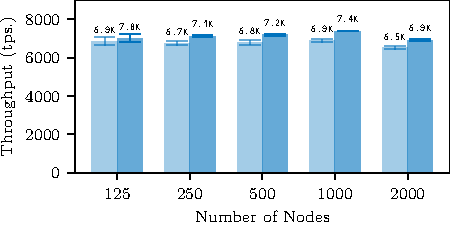
\includegraphics[width=\linewidth]{figures/thr-ava.pdf}
\captionof{figure}{Débit transactionnel en fonction de la taille du réseau. Chaque paire de barres est produite avec
une taille de batch de 20 et 40, de gauche à droite.}
\label{fig:eval-thr}
\end{figure}

\begin{figure}
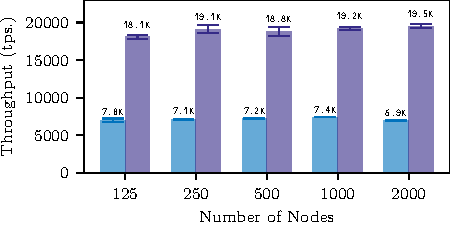
\includegraphics[width=\linewidth]{figures/thr-raw.pdf}
\captionof{figure}{Débit transactionnel pour une taille de batch de 40, avec (gauche) et sans (droite) vérification
de la signature.}
\label{fig:eval-thr-raw}
\end{figure}

\subsection{Mise à l'échelle}

Afin d'observer la manière dont le système passe à l'échelle en terme de nombre de noeuds participant au consensus
{\sysname}, nous effectuons des expériences en gardant des paramètres identiques tout en faisant varier le
nombre de noeuds de 125 jusqu'à 2000.

La Figure~\ref{fig:eval-thr} montre que le débit global se dégrade d'environ $1.34\%$ à 6909 tps lorsque le
réseau augmente d'un facteur 16 pour atteindre $n = 2000$. Cette dégradation est mineure si on la compare au
taux d'augmentation du réseau. Notez que l'axe X est logarithmique.

Avalanche tire sa bonne mise à l'échelle de plusieurs sources\,: premièrement en maintenant un ordre partiel qui
capture uniquement les relations entre les dépenses ce qui permet une meilleure parallélisation qu'un journal
BFT répliqué classique qui traite toutes les transactions de manière linéaire\,; deuxièmement l'absence de dirigeant
permet d'éviter les goulets d'étranglement\,; et finalement le nombre de messages que chaque noeud doit gérer par
décision est $O(k)$ et n'augmente pas au fur et à mesure que le réseau s'agrandit.

\subsection{Engorgement dû à la cryptographie}

Nous examinons ensuite où se situent les goulets d'étranglement dans notre implémentation.
La barre violette à la droite de chaque groupe dans la Figure~\ref{fig:eval-thr-raw} montre le débit
d'Avalanche lorsque la vérification des signatures est désactivée. Les débits s'améliorent d'environ 2.6x, par
par rapport à la barre bleue sur la gauche.
Cela révèle que le surplus de calcul dû à la vérification cryptographique est le principal goulet d'étranglement
de l'implémentation de notre système. On peut pallier ce problème en déléguant la vérification des transactions
à un GPU\@. Même en l'absence d'une telle optimisation, 7K tps dépasse de loin ce qui existe en matière de blockchain.

\subsection{Latence}

\begin{figure}
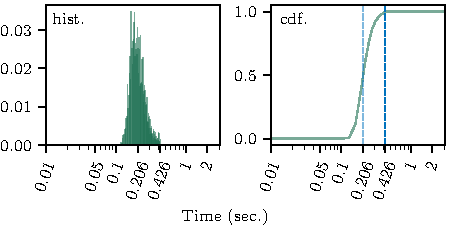
\includegraphics[width=\linewidth]{figures/lat.pdf}
\captionof{figure}{Distribution de la latence de transaction pour $n = 2000$. L'axe X représente la latence
    de transaction en secondes sur une échelle logarithmique, tandis que l'axe Y est la portion des transactions
    qui tombe dans la période de confirmation (normalisée à $1$). L'histogramme de toutes les latences de transaction
    pour un client est visible sur la gauche avec $100$ bins, et son CDF visible sur la droite.}
\label{fig:eval-lat1}
\end{figure}

La latence d'une transaction est le temps écoulé à partir du moment où elle est soumise au réseau jusqu'à ce qu'elle
soit confirmée et donc acceptée par le réseau.

La Figure~\ref{fig:eval-lat1} représente un histogramme montrant la distribution des latences en utilisant la
même configuration que pour les mesures de débits à partir de 2000 noeuds. L'axe X représente le temps en secondes
tandis que l'axe Y est la portion des transactions qui sont finalisées dans la période de temps correspondante.
Cette figure met également en avant la Fonction de Distribution Cumulée (CDF) en accumulant le nombre de
transactions finalisées sur la période.

Cette expérience démontre que la plupart des transactions sont confirmées en moins de 0.3 secondes environ.
La majorité des latences se trouve aux alentours des 206 ms avec une variance relativement faible, ce qui
indique que les noeuds convergent sur la décision finale en tant que groupe environ au même moment. La deuxième
ligne verticale montre la latence maximale observée, qui se situe aux alentours des 0.4 secondes.

La Figure~\ref{fig:eval-lat2} montre la latence de transaction pour un nombre variable de noeuds. Les arêtes
horizontales des boîtes représentent respectivement du bas vers le haut le minimum, le premier quartile, la médiane,
le troisième quartile, et le maximum de latence. En définitive, les données expérimentales montrent que la latence
médiane est plus ou moins indépendante de la taille du réseau.

\begin{figure}[h]
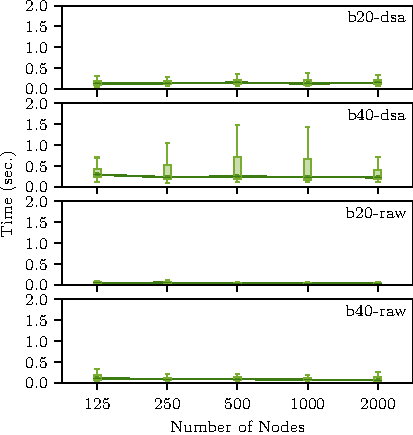
\includegraphics[width=\linewidth]{figures/lat2.pdf}
\captionof{figure}{Latence de transaction en fonction de la taille du réseau. ``b'' indique la taille de batch et
``raw'' est l'occurence sans la vérification des signatures.}
\label{fig:eval-lat2}
\end{figure}

\subsection{Clients malveillants}
\label{sec:evaluation-misbehaving}
\begin{figure}
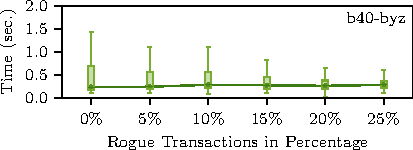
\includegraphics[width=\linewidth]{figures/lat3.pdf}
\captionof{figure}{Latence en fonction du taux de transactions malveillantes.}
\label{fig:eval-lat3}
\end{figure}

Nous évaluons ensuite comment des transactions conflictuelles générées par des clients malveillants effectuant des
double dépenses sur des sorties non dépensées peuvent affecter la latence des transactions légitimes créées par
des clients corrects. Nous adoptons une stratégie qui simule des clients malveillants où une fraction (de $0\%$ à $25\%$)
des transactions en attente sont en conflit avec d'autres transactions existantes.

Le processus client effectue ceci en désignant des flux de transactions contenant des double dépenses parmi toutes
les transactions simulées en attente, et envoie les transactions conflictuelles vers différents noeuds. Nous utilisons
pour cela les mêmes paramètres avec $n = 1000$ comme dans les expériences précédentes, et nous mesurons uniquement
le débit et la latence des transactions confirmées.

La latence d'{\sysname} est seulement légèrement influencée par les clients malveillants, comme le montre la
Figure~\ref{fig:eval-lat3}. Étonnamment, la latence maximale baisse légèrement lorsque le pourcentage de transactions
conflictuelles augmente. Ce comportement s'explique par le fait que lorsqu'on introduit de telles transactions, le débit
\emph{effectif} est réduit et soulage donc la charge du système.

Cette observation est confirmée par la figure~\ref{fig:eval-thr2} qui montre que le débit (de transactions légitimes)
decroît avec le taux de transactions conflictuelles. De plus, la baisse du débit apparaît proportionnelle au nombre de
clients malveillants, ce qui démontre que les attaques potentielles ne bénéficient pas d'un effet de levier.

\begin{figure}
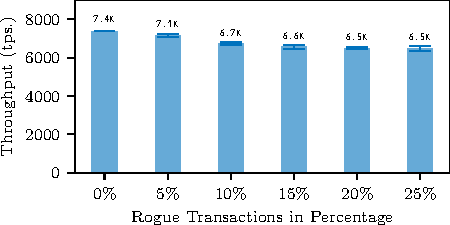
\includegraphics[width=\linewidth]{figures/thr-byz.pdf}
\captionof{figure}{Débit de transactions en fonction du taux de transactions conflictuelles.}
\label{fig:eval-thr2}
\end{figure}

\subsection{Géo-réplication}

\begin{figure}
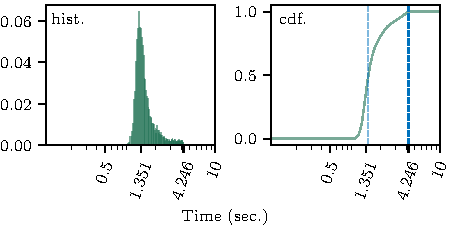
\includegraphics[width=\linewidth]{figures/lat4.pdf}
\captionof{figure}{Histogramme de latence/CDF pour $n = 2000$ réparties dans 20 villes.}
\label{fig:eval-lat4}
\end{figure}

L'expérience suivante place le système dans l'émulation d'un scénario géo-répliqué, modélisé sur le même scénario
détaillé dans un travail préliminaire~\cite{GiladHMVZ17}.
Nous avons sélectionné 20 villes majeures qui semblent être localisées à proximité d'un nombre conséquent de noeuds
Bitcoin joignables, d'après ~\cite{bitnodes2018}. Ces villes couvrent l'Amérique du Nord, l'Europe, l'Asie occidentale,
l'Asie orientale, l'Océanie, et incluent également les 10 villes où l'on trouve le plus grand nombre de noeuds
joignables. Nous utilisons les données de latence obtenues depuis~\cite{wondernetworkping2018} et nous émulons
la latence des paquets réseau dans le noyau Linux en utilisant les commandes \texttt{tc} et \texttt{netem}.
2000 noeuds sont distribués équitablement parmi toutes les villes, sans émuler de latence supplémentaire entre les
noeuds d'une même ville. Comme pour l'évaluation d'Algorand, nous limitons aussi la bande passante par processus
à 20 mégabits par seconde dans le but de simuler des paramètres à l'échelle d'internet d'un réseau comportant de
nombreux liens. Nous assignons ensuite un processus client à chaque ville, qui génère 400 transactions sortantes
par ville à tout moment.

Dans ce scénario, Avalanche atteint un débit de transactions moyen de 3401 tps, avec un écart type de 39 tps. Comme
le montre la Figure~\ref{fig:eval-lat4}, la latence de transaction médiane est de 1.35 secondes, avec une latence
maximale de 4.25 secondes. Nous supportons également le code initial de Bitcoin pour les transactions, qui dans ce
cas donne un débit de 3530 tps avec $\sigma = 92$ tps.

\subsection{Comparaison avec d'autres systèmes}

Même s'il existe une abondance de protocoles blockchain et de cryptomonnaies, la plupart d'entre eux présentent
une ébauche de leur protocole sans proposer d'implémentation pratique ou de résultats d'évaluation. En outre, parmi
ceux qui proposent effectivement des résultats, la plupart ne sont pas évalués dans des conditions réalistes ou à
grande échelle (des centaines de milliers de noeuds complets participant au consensus).

En conséquent, nous choisissons Algorand et Conflux pour notre étude comparative. Algorand, Conflux et Avalanche
sont tous fondamentalement différents dans leur conception. L'algorithme de consensus par comité
d'Algorand repose sur un accord byzantin basé sur un quorum, et Conflux supplémente le consensus de Nakamoto par une
structure de type Graphe Acyclique Orienté (DAG) pour permettre un meilleur débit, tandis qu'Avalanche appartient à
une nouvelle famille de protocoles basés sur la méta-stabilité. Par ailleurs, nous utilisons
Bitcoin~\cite{nakamoto2008bitcoin} comme base technique.

Les évaluations d'Algorand et d'Avalanche reposent toutes deux sur un réseau décisionnel de 2000 noeuds sur EC2.
Notre évaluation se fait sur des instances \texttt{c5.large} partagées, tandis qu'Algorand utilise des instances
\texttt{m4.2xlarge}\@. Ces deux plateformes sont très similaires à l'exception d'un léger avantage en terme de
fréquence CPU pour le \texttt{c5.large}, qui au final n'est que partiellement utilisé puisque nos processus ne
consomment que $30\%$ de temps processeur lors de ces expériences. Les paramètres de sécurité choisis pour nos
expériences garantissent une probabilité de violation de sécurité en dessous de $10^{-9}$ en présence de
$20\%$ de noeuds byzantins, en comparaison de l'évaluation Algorand qui garantit une probabilité de violation en dessous
de $5 \times 10^{-9}$ avec $20\%$ de noeuds byzantins.

Ni Algorand ni Conflux ne prennent en compte le surplus de calcul lié à la vérification cryptographique dans leurs
études. Leurs évaluations utilisent des blocs qui contiennent des mégaoctets de données factices et présentent les
mesures de débit en mégaoctets ou gigaoctets par heure. Nous utilisons donc la taille moyenne d'une transaction
Bitcoin, 250 octets, pour en déduire leurs débits de transactions. Par contraste, nos expériences transportent des
données de transactions réelles et prennent entièrement en compte le temps de calcul des vérifications cryptographiques.

Le débit de transactions est de 3-7 tps pour Bitcoin, 874 tps pour Algorand (avec des blocs de 10 mégaoctets), 3355 tps
pour Conflux (le papier fait mention d'un débit 3.84 fois supérieur au débit d'Algorand dans les mêmes conditions).

En comparaison, {\sysname} obtient constamment plus de 3400 tps sur un réseau allant jusqu'à 2000 noeuds
sans aucun comité de décision ni preuve de travail. Pour ce qui est de la latence, une transaction est confirmée
après 10--60 minutes pour Bitcoin, environ 50 secondes pour Algorand, 7.6--13.8 minutes avec Conflux, et 1.35 secondes
pour {\sysname}.

Avalanche se comporte bien mieux qu'Algorand à la fois en terme de débit et de latence étant donné qu'Algorand utilise une
fonction aléatoire vérifiable pour élire ses comités, et maintient un journal ordonné pendant qu'{\sysname} établit
un ordre partiel uniquement. Bien que l'entité à la tête d'Algorand soit anonyme et change continuellement, elle reste
néanmoins basée sur un dirigeant unique qui pourrait être un facteur limitant pour le passage à l'échelle, tandis
qu'{\sysname} n'est pas contrôlé par une entité unique.

Avalanche a un débit similaire à Conflux, mais sa latence est 337--613 fois meilleure. Conflux utilise également une
structure DAG pour amortir le coût du consensus et augmenter le débit de transactions, cependant il est toujours ancré
sur un consensus de Nakamoto (PoW) le rendant incapable de confirmer des transactions instantanément comme le fait
Avalanche.

Dans un système à base de blockchain, on ne peut généralement améliorer le débit des transactions qu'aux dépens de la
latence à travers le regroupement par batchs. Le vrai facteur limitant au niveau de la performance est le nombre de
décisions qu'un système est en mesure de prendre en une seconde, et ce paramètre est fondamentalement limité soit par
l'accord byzantin ($\mathrm{BA}^{*}$) chez Algorand soit par le consensus de Nakamoto pour Conflux.

